\documentclass[tikz,border=10pt]{standalone}
\usetikzlibrary{shapes.geometric, arrows.meta}

\tikzset{
    block/.style = {rectangle, draw, fill=blue!20, 
        text width=5em, text centered, rounded corners, minimum height=4em},
    line/.style = {draw, -Stealth, thick},
    dashedline/.style = {dashed, draw, -Stealth, thick},
    node distance=3cm,
}

\begin{document}
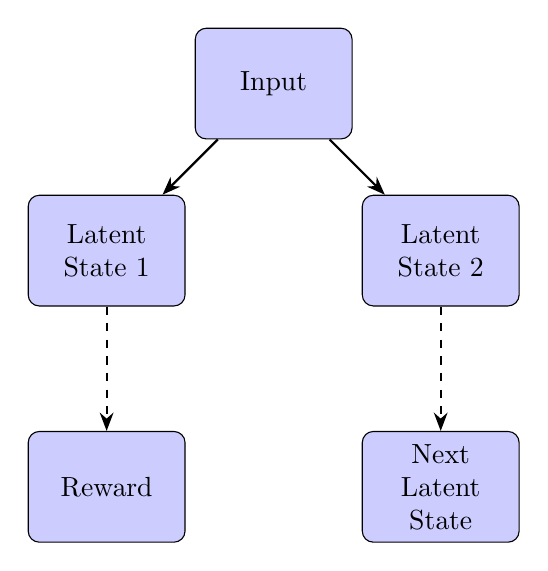
\begin{tikzpicture}[auto]

    % Nodes
    \node [block] (input) {Input};
    \node [block, below left of=input] (latent1) {Latent State 1};
    \node [block, below right of=input] (latent2) {Latent State 2};
    \node [block, below of=latent1] (reward) {Reward};
    \node [block, below of=latent2] (nextState) {Next Latent State};

    % Edges
    \path [line] (input) -- (latent1);
    \path [line] (input) -- (latent2);
    \path [dashedline] (latent1) -- (reward);
    \path [dashedline] (latent2) -- (nextState);

\end{tikzpicture}
\end{document}